\documentclass[c]{beamer}

\usetheme{CambridgeUS}
\usecolortheme{dolphin}
\setbeamercolor{footline}{fg=white, bg=black}

%%%%%    set the bullet style to rectangles   %%%%%
\useinnertheme{rectangles}

%%% change default style of beamer bibliography %%%
\setbeamertemplate{bibliography item}{\insertbiblabel}

%%%%%%%%   remove bottom navigation bar   %%%%%%%%%
\beamertemplatenavigationsymbolsempty
\usepackage{ragged2e}       %justification
\usepackage{graphicx} 		% Allows including images
\usepackage[table]{xcolor}
\usepackage{fixltx2e} 		% need to use the \textsubscript{} command
\usepackage[font=scriptsize]{caption}
\usepackage[font=scriptsize]{subcaption}
\usepackage{algorithmic} 	% need to write some algorithms
\usepackage{amsmath}		% need to write some equations

\title[Effective Machine Learning with Cloud TPU] 	% (optional, only for long titles, this will be displayed as footer in slides)
{Effective Machine Learning with Cloud TPU}

\author[ATHUL K S] % (optional, for multiple authors)
{\Large ATHUL K S}
\institute[GECW]
{\large
	ROLL NO. 16\\[5pt]
	S\textsubscript{6} B.Tech CSE\\ \vspace{3mm}
	Guided by : Ms. Bintu Balachandran (Assistant Professor, CSE Dept)\vspace{3mm}
	Government Engineering College, Wayanad\\[5pt]
}
\date[]{\today}

\subject{High processing computer \& Machine learning}

%%%%%%%%%%%%%%%%%%%%%%%%%%%%%%%%%%%%%%%%%%%%%%%%%%%%%%%%%%%%%%%%%%%%%%%%
%% Uncomment this to include a table of contents before every section %%
%%%%%%%%%%%%%%%%%%%%%%%%%%%%%%%%%%%%%%%%%%%%%%%%%%%%%%%%%%%%%%%%%%%%%%%%

%\AtBeginSection[]
%{
%	\begin{frame}[plain]{Outline}
%	\tableofcontents[currentsection]
%	\end{frame}
%}

\begin{document}
	% this one gives an animation effect to every \item s 
	
	\frame[plain]{\titlepage}

	%%%%%%%%%%%%%%%%%%%%%%%%%%%%%%%%%%%%%%
	
	\begin{frame}[plain]{Overview}
		\tableofcontents
	\end{frame}

	%%%%%%%%%%%% Introduction %%%%%%%%%%%%

	\section{INTRODUCTION}
	
	\begin{frame} [c]
		\frametitle{Introduction}
		\begin{itemize}
		\justifying
			\item Major ML progress over past several year.
			\newline
			 \item There's been a tremendous amount of machine learning progress over the past several years. The number of research publications on arvix is growing faster than Moore's law. Like 50 new machine learning papers every day and tremendous increase in accuracy.
\newline
			\item Many architects believe that major improvements in cost-energy performance must now come from domain-specific hardware.
		\end{itemize}			
	\end{frame}
        %%%%%%%%%%%%%%%%%%%%%%%%%%%%%%%%%%%%%%%%%%
    \begin{frame} [c]
        \frametitle{\centerline{ML Arvix papers per year}}
        \begin{figure}
            \centering
           % 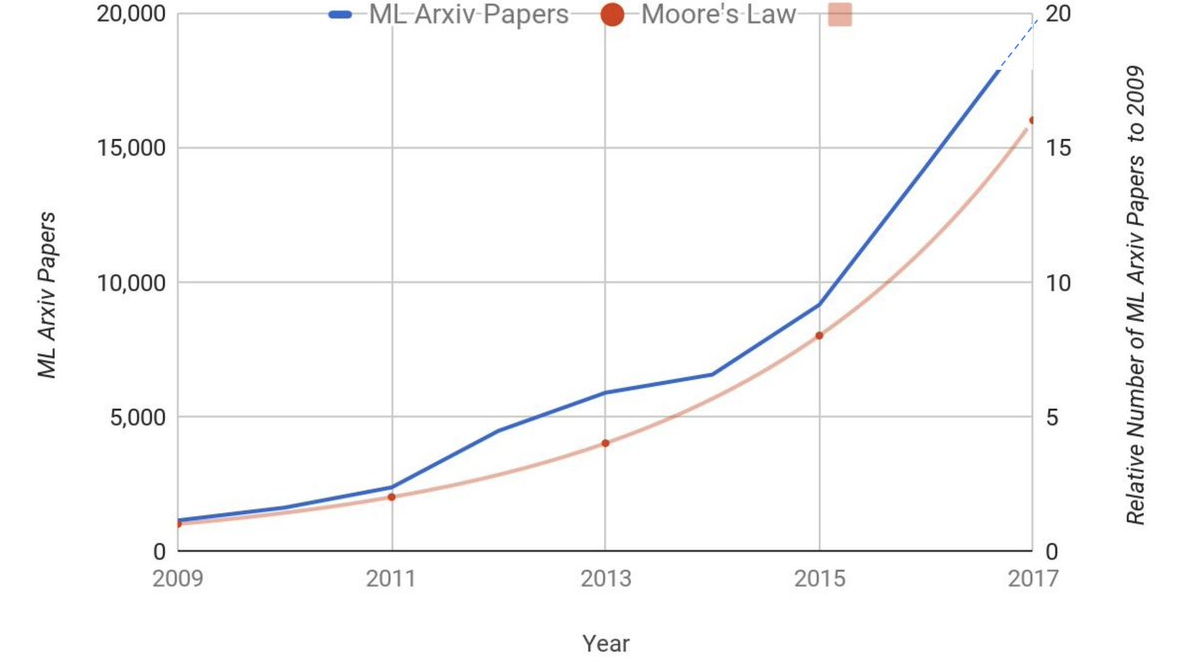
\includegraphics[width=7cm]{images/1arvix.png}
            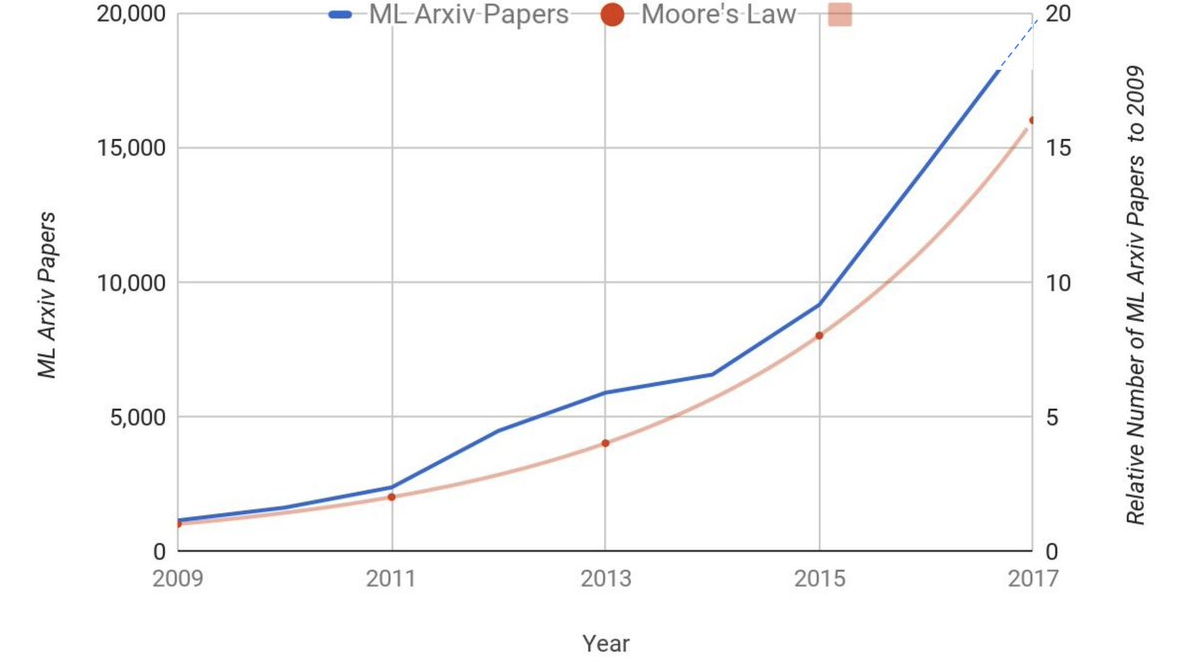
\includegraphics[scale=.36]{images/1arvix.png}
            \caption{1. Papers published }
            \label{graph: Papers Published}
        \end{figure}
    \end{frame}
        %%%%%%%%%%%%%%%%%%%%%%%%%%%%%%%%%%%%%%%%%%
\begin{frame} [c]
        \frametitle{\centerline{Rapid Accuracy Improvement}}
        \begin{figure}
            \centering
           % 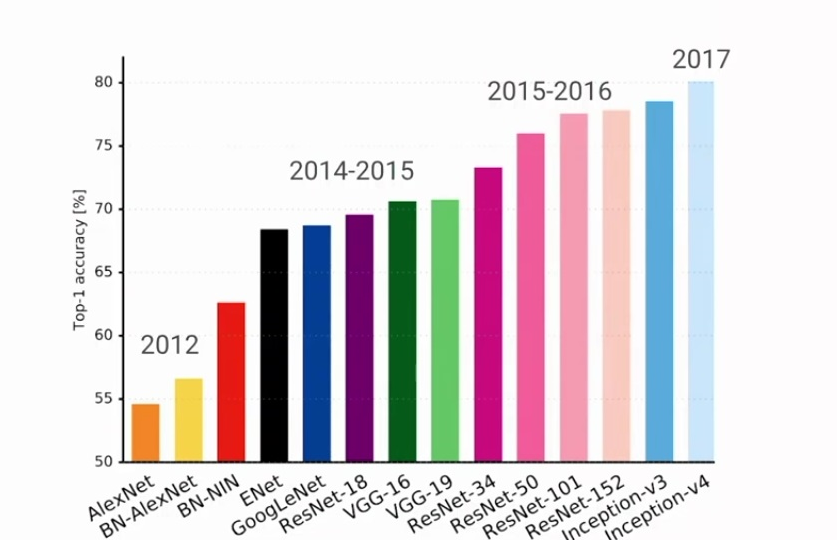
\includegraphics[width=7cm]{images/2accuracy.png}
            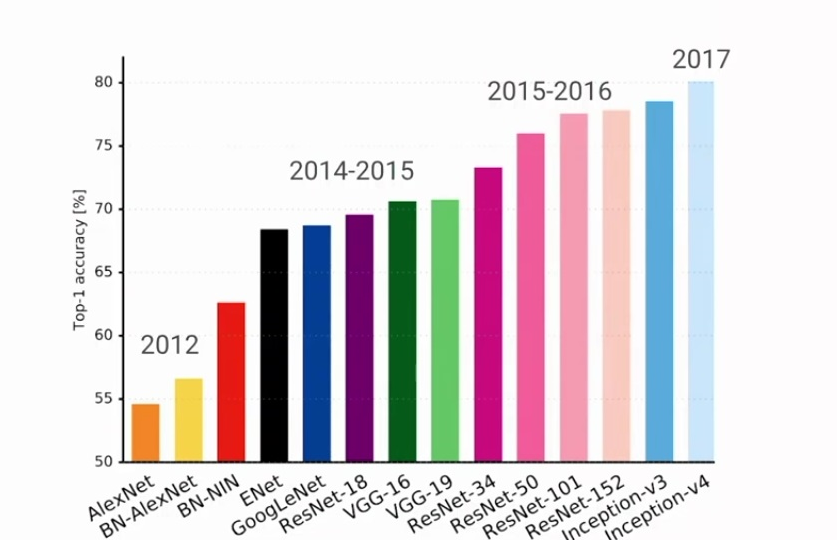
\includegraphics[scale=.45]{images/2accuracy.png}
            \caption{2.Accuracy in Machine Learning}
            \label{graph: Accuracy in MAchine Learning}
        \end{figure}
    \end{frame}
	%%%%%%%%%%%%%%%%%%%%%%%%%%%%%%%%%%%%%
	\begin{frame} [c]
		\frametitle{\centerline {\small{Challenge : Increasing Complexity and Computational cost}}}
		\begin{figure}[ht]
  {\begin{minipage}[t]{125pt}
    \includegraphics[height=100pt,width=150pt]{test}
    	\begin{itemize}
		\justifying
			\item {\small As these models get more accurate they tend to be larger trained on larger data sets and that means that you need more computation both to train the model on the data set and then eventually to run it.}
		\end{itemize}		
  \end{minipage}}
  \hfill
  {\begin{minipage}[t]{205pt}
    \includegraphics[height=60pt,width=150pt]{test}
    
           % \includegraphics[width=7cm]{images/3challange.png}
                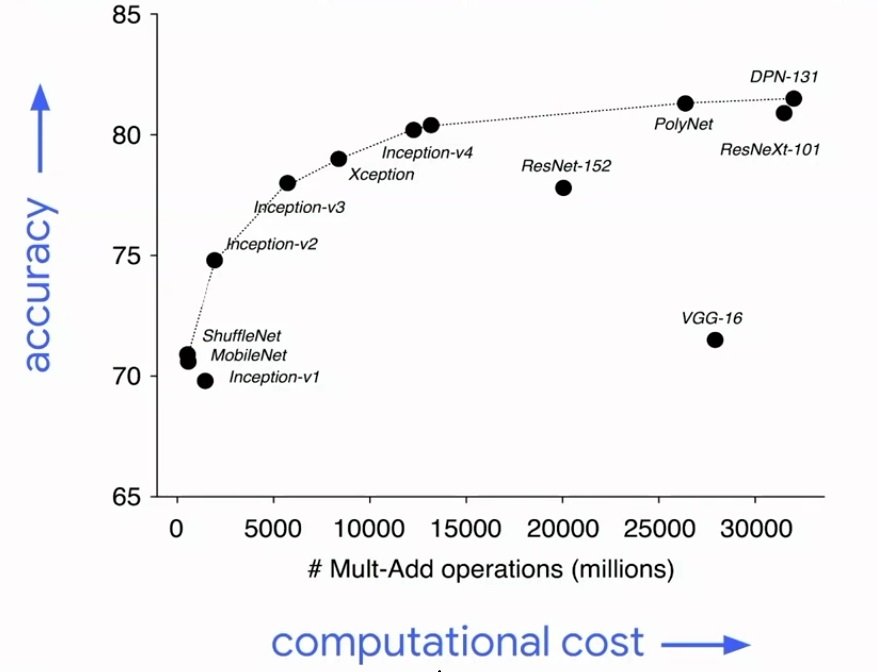
\includegraphics[scale=.32]{images/3challenge.png}
            \caption
            {3. computational cost Vs accuracy}
            \label{graph: computational cost Vs accuracy}
        
  \end{minipage}}
\end{figure}
	\end{frame}
	%%%%%%%%%%%%%%%%%%%%%%%
	
\section{EVOLUTION}
	\begin{frame} [c]
		\frametitle{Evolution}
        \begin{itemize}
        \justifying
              \item \large TPUv1 : Google’s first Tensor Processing Unit (TPU)
           \end{itemize} 
           \begin{figure}
            \centering
           % 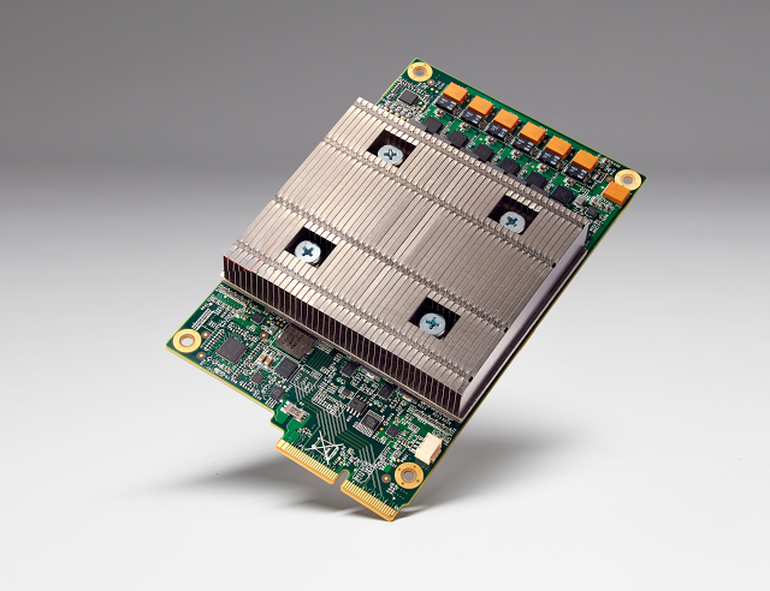
\includegraphics[width=7cm]{images/4tpu.png}
            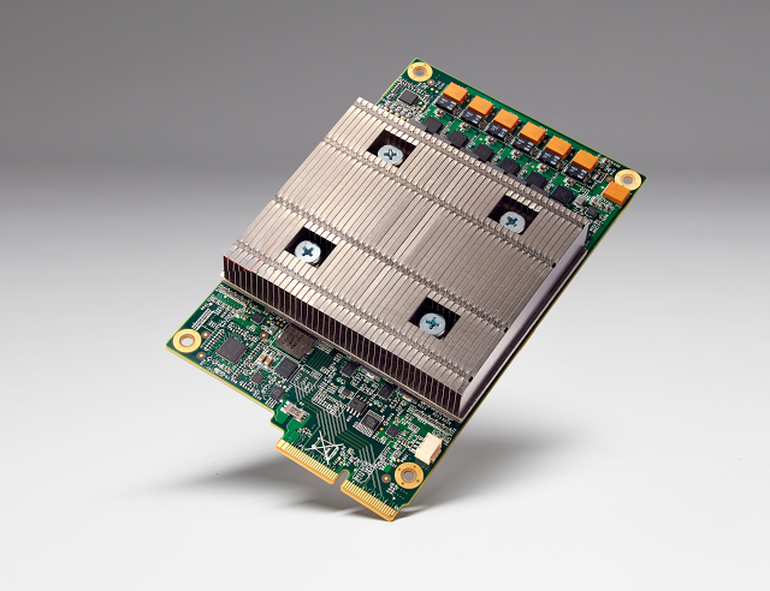
\includegraphics[scale=.38]{images/4tpu.png}
            \caption{4. TPUv1}
            \label{fig:TPUv1}
        \end{figure}
	\end{frame}
        %%%%%%%%%%%%%%%%%%%%%%%%%%%%%%%%%%%%%%%	
        
	\begin{frame} [c]
		\frametitle{Evolution}
        \begin{itemize}
        \justifying
              \item \large TPUv2 : Cloud TPU
           \end{itemize} 
           \begin{figure}
            \centering
           % \includegraphics[width=7cm]{images/5cloudtputpu.png}
            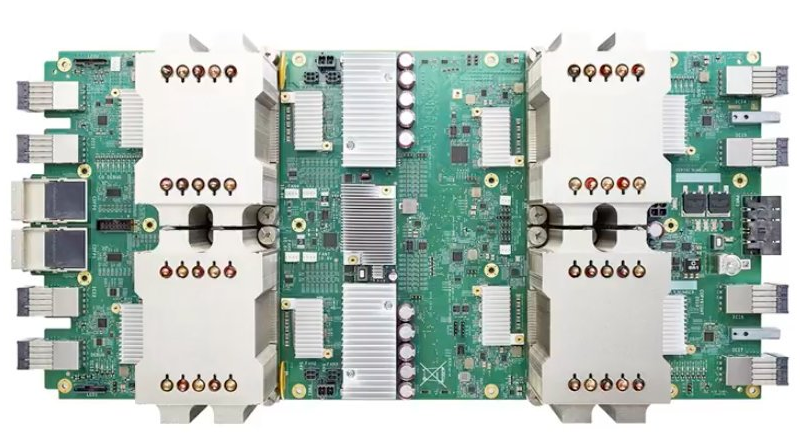
\includegraphics[scale=.4]{images/5cloudtpu.png}
            \caption{5. TPUv2}
            \label{fig:TPUv2}
           \end{figure}
	\end{frame}
	%%%%%%%%%%%%%%%%%%%%%%%%%%%%%%%%
	  
	\begin{frame} [c]
		\frametitle{Evolution}
        \begin{itemize}
        \justifying
              \item \large Cloud TPUv2 pod
           \end{itemize} 
           \begin{figure}
            \centering
           % \includegraphics[width=7cm]{images/6cloudtpupod.png}
            \includegraphics[scale=0.14]{images/6cloudtpupod.png}
            \caption{6. Cloud TPUv2 pod}
            \label{fig:Cloud TPUv2 pod}
           \end{figure}
	\end{frame}
	%%%%%%%%%%%%%%%%%%%%%%%%%%%%%%%%%%
	\begin{frame}[h]
	\frametitle{Evolution}
	\begin{itemize}
	    	\justifying
			\item {\footnotesize The TPUv3 chip runs so hot that for first time Google has introduced liquid cooling in its data centers.}
\item{\footnotesize TPUv3 pod is eight times more powerful than a TPUv2 pod.}
\newline
	\end{itemize}
	\begin{figure}[h]
 \hfill
\begin{subfigure}{0.40\textwidth}
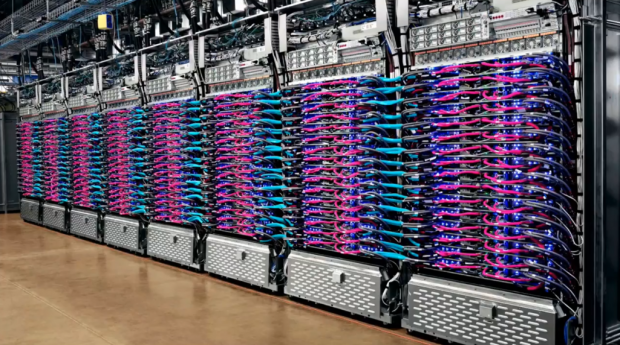
\includegraphics[width=1.05\linewidth,height=3.3cm]{images/7atpuv3pod.png} 
\caption{ TPUv3 pod}
\label{fig:TPUv3 pod}
\end{subfigure}
\space
\space
\space
\begin{subfigure}{0.5\textwidth}
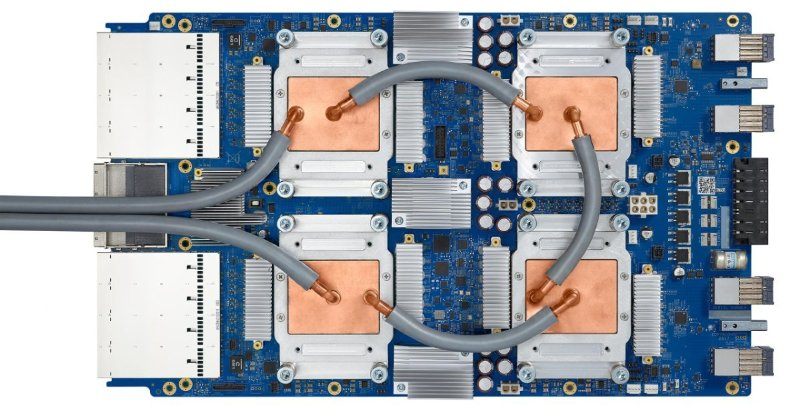
\includegraphics[width=.95\linewidth,height=3.3cm]{images/7btpuv3.png}
\caption{TPUv3 Chip}
\label{fig:TPUv3 Chip}
\end{subfigure}
 
\caption{7. TPUv3}
\label{fig:TPUv3}
\end{figure}
	\end{frame}
	%%%%%%%%%%%%%%%%%%%%%%%%%%
	\begin{frame} [c]
		\frametitle{Relentless Effort}
		\begin{figure}[t]
  {\begin{minipage}{58.3pt}
    \includegraphics[height=100pt,width=150pt]{test}
    TPUv1\newline
{\small  (2015)}
\newline
\newline
\newline
\newline
\newline
Cloud TPU\newline
{\small  (2017)}
\newline
\newline
\newline
\newline
TPU pod\newline
{\small  (2017)}
  \end{minipage}}
  \hfill
  {\begin{minipage}{145pt}
    \includegraphics[height=100pt,width=150pt]{test}
     \begin{center}
		 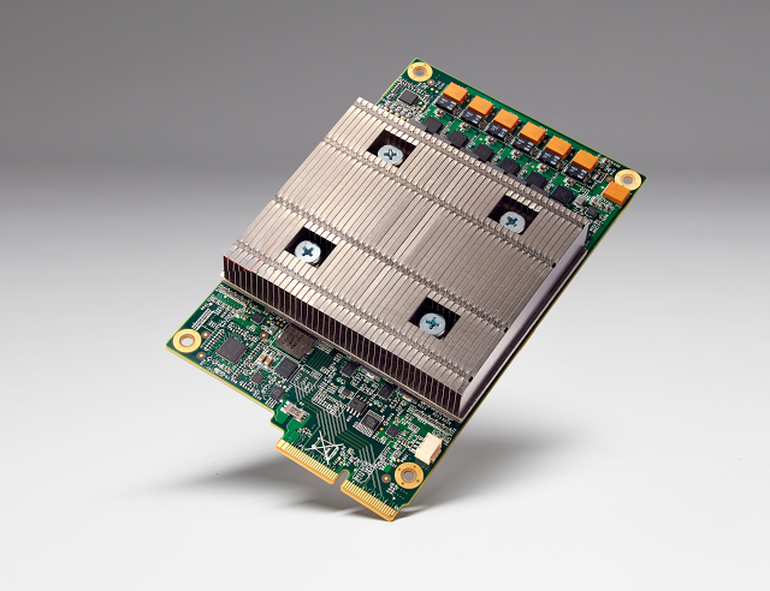
\includegraphics[scale=.16]{images/4tpu.png}
           \label{fig: TPUv1}
          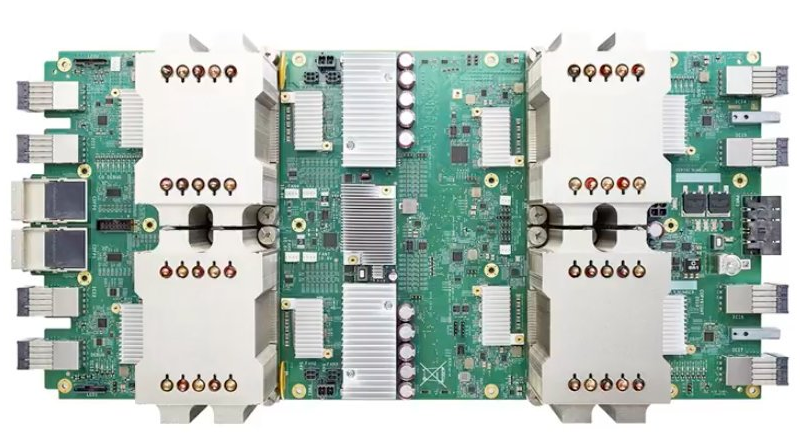
\includegraphics[scale=.2]{images/5cloudtpu.png}
            \label{fig: cloud TPU}
            \includegraphics[scale=.065]{images/6cloudtpupod.png}
              \label{fig: TPU pod}
            \end{center}
  \end{minipage}}
   {\begin{minipage}{120pt}
    \includegraphics[height=100pt,width=150pt]{test}
    \newline
    \newline
   {\small \space 92 TeraFlops \newline
   \space \space Inference only
   \newline
   \newline
\newline
\newline
\space \space180 TeraFlops\newline 
\space \space 64 GB HBM\newline
\space \space Training and inference
\newline
\newline
\newline
\space  \space11.5 PetaFlops\newline
\space  \space 4TB HBM\newline
\space \space 2D toroidal mesh network \newline
\space \space Training and inference\newline}

  \end{minipage}}
\end{figure}
	\end{frame}
	
		%%%%%%%%%%%%%%%%%%%%%%%%%%%%%%%%%%
		\begin{frame} [c]
		\frametitle{Relentless Effort}
		\begin{figure}[t]
{\begin{minipage}[t]{65pt}
    \includegraphics[height=100pt,width=150pt]{test}
    \newline
    \newline
    TPUv3\newline
{\small  (2018)}
\newline
\newline
\newline
\newline
\newline
TPUv3 pod\newline
{\small  (2018)}
\newline
\newline
\newline
\newline

  \end{minipage}}
  \hfill
  {\begin{minipage}[t]{145pt}
    \includegraphics[height=100pt,width=150pt]{test}
     \begin{center}
		 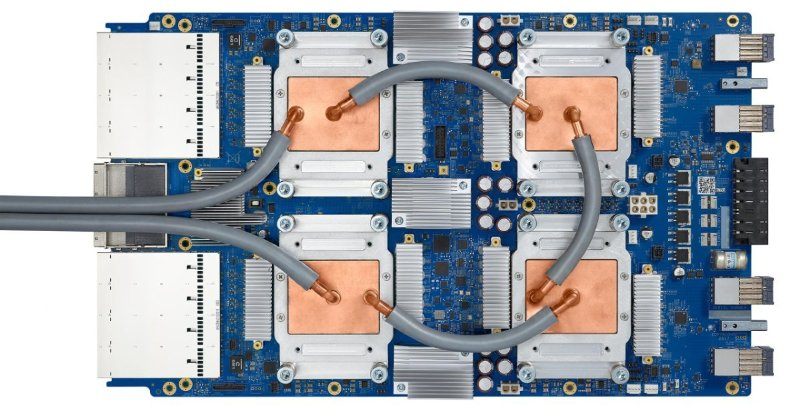
\includegraphics[scale=.2]{images/7btpuv3.png} 
		 \newline
		 \newline
		 \label{fig: TPUv3}
          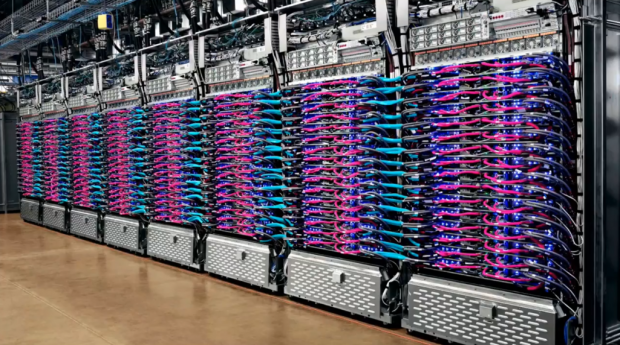
\includegraphics[scale=.3]{images/7atpuv3pod.png}            \label{fig: Cloud TPUv3 pod}
            \end{center}
  \end{minipage}}
   {\begin{minipage}[t]{120pt}
    \includegraphics[height=100pt,width=150pt]{test}
    \newline
    \newline
   {\small \space 420 terraflops
 \newline
   \space \space 128 GB HBM\newline
    New chip architecture
   \newline
\newline
\newline
\space \space $>$100 petaflops\newline 
\space \space More than 8x the performance than a TPUv2 Pod\newline
\space \space \newline
\newline
\newline
\newline}

  \end{minipage}}
\end{figure}
	\end{frame}
	
		%%%%%%%%%%%%%%%%%%%%%%%%%%%%%%%%%%
		

\section{ARCHITECTURE}
	\begin{frame}
	\frametitle{Architechture: TPUv1}
			\begin{figure}[ht]
  {\begin{minipage}[t]{150pt}
    \includegraphics[height=100pt,width=150pt]{test}
    	\begin{itemize}
		\justifying
		{\small	\item The matrix unit : 65,536 (256x 256)
            \item700MHz clock rate
            \item Peak 92 operations per scond 
            \item 4MiB of on-chip Accumulator memory
            \item 24 MiB of on chip Unified Buffer (activation memory). 3.5 X  as much on-chip memory Vs GPU
            \item Two 2133MHz DDR3 channels
            \item 8GiB of off-chip weight DRAM memory
            \item CISC}

		\end{itemize}		
  \end{minipage}}
  \hfill
  {\begin{minipage}[t]{180pt}
    \includegraphics[height=60pt,width=150pt]{test}
    
           % \includegraphics[width=7cm]{images/3challange.png}
                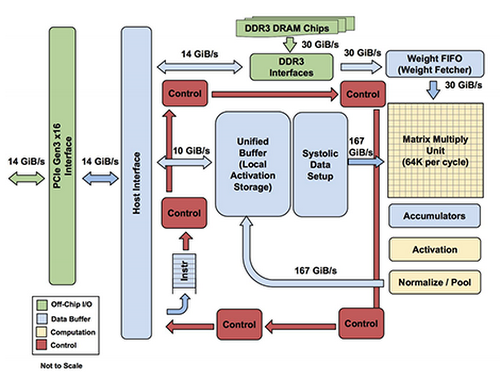
\includegraphics[scale=.5]{images/8tpuv1.png}
            \caption
            {8. schematic diagram of TPUv1}
            \label{graph: computational cost Vs accuracy}
        
  \end{minipage}}
\end{figure}
    \end{frame}
  %%%%%%%%%%%%%%%%%%%%%%%%%%%%%%%%%%%%%%%%%%%%%%%%%%%%%%%  
  \begin{frame}[t]
  \frametitle{Architecture TPUv1}
   \textbf {Mathematical Operations required for Neural Network Inference} \newline
   \begin{table}
  {\centering
\begin{tabular}{ |p{5.5cm}|p{5.5cm}|  }
\hline
\multicolumn {2}{|c|}{}\\
\multicolumn {2}{|c|}{\large Instructions for Neural Network Inference} \\ 
\multicolumn {2}{|c|}{}\\
\hline
\textbf{TPU Instructions} & \textbf{Functions}  \\
\hline
Read\_Host\_Memory & Read data from memory \\
\hline
Read\_Weights & Read weight from memory\\
\hline
MartrixMultiply/Convolve & Multiply or convolve with the data and weights,accumulate the result\\
\hline
Activate & Applyactivation function \\
\hline
Write\_Host\_Memory & Write result to memory \\
\hline
\end{tabular}}
	\caption{1. Instructions and functions}
	 \label{tab:table1}
	\end{table}
  \end{frame}
  %%%%%%%%%%%%%%%%%%%%%%%%%%%%%%%%%%%%%%%%%%%%%%%%%%%%%%
  \begin{frame} [c]
  \frametitle{Architechture : Cloud TPU}
  \begin{figure}
   \centering
           % \includegraphics[width=7cm]{images/6cloudtpupod.png}
            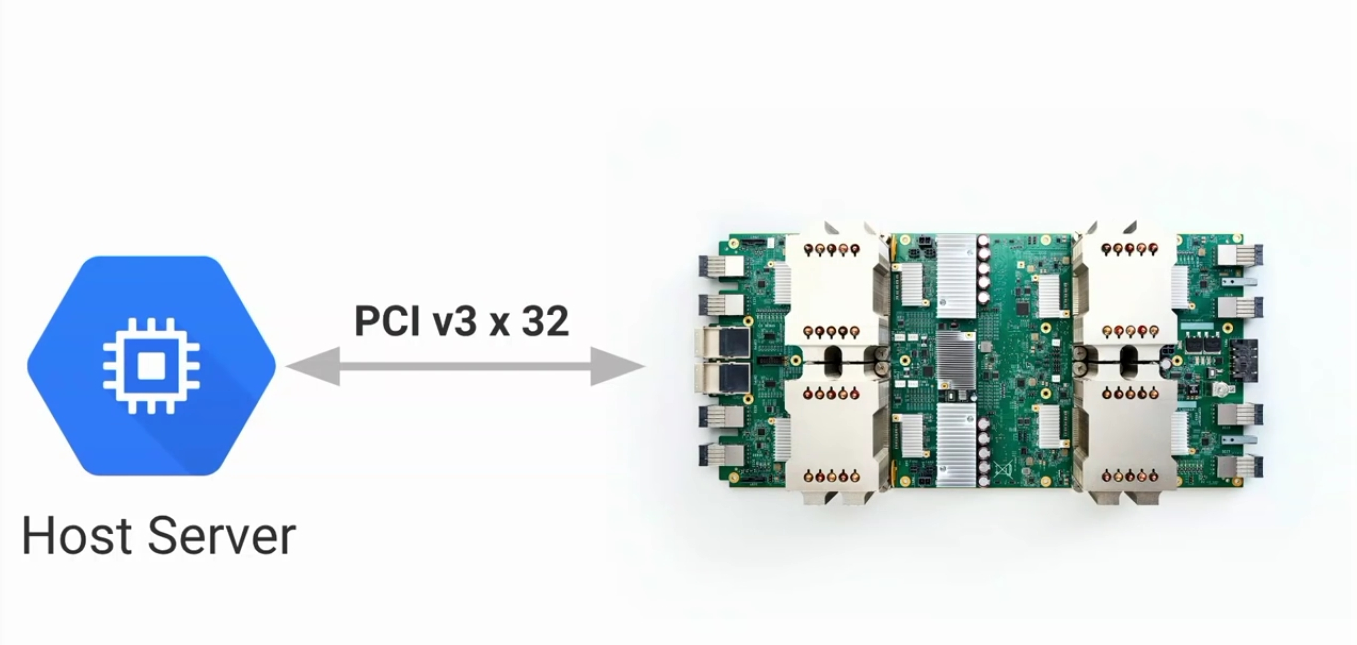
\includegraphics[scale=0.225]{images/9cloudtpu.png}
            \caption{6. Cloud TPU}
            \label{fig:Cloud TPU}
  \end{figure}
  \begin{itemize}
     {\small \item 180 TeraFlops of computation
\item 64 GB of HBM memory
\item2400 GB/s mem
\item Designed to be connected together into larger configuration
\item CISC}

  \end{itemize}
  \end{frame}
  %%%%%%%%%%%%%%%%%%%%%%%%%%%%%%%%%%%%%%%%%%%%%%%%%%%%%%
  \begin{frame} [c]
  \frametitle{Architechture : Cloud TPU}
			\begin{figure}[ht]
  {\begin{minipage}[t]{120pt}
    \includegraphics[height=100pt,width=150pt]{test}
    	\begin{itemize}
		\justifying
		{\small \item16 GB of HBM
\item 600 GB/s mem
\item vector units: 32b float
\item MXU: 32b float accumulation but reduced precision for multipliers
\item 45TFLOPS
	}

		\end{itemize}		
  \end{minipage}}
  \hfill
  {\begin{minipage}[t]{215pt}
    \includegraphics[height=60pt,width=150pt]{test}
    
                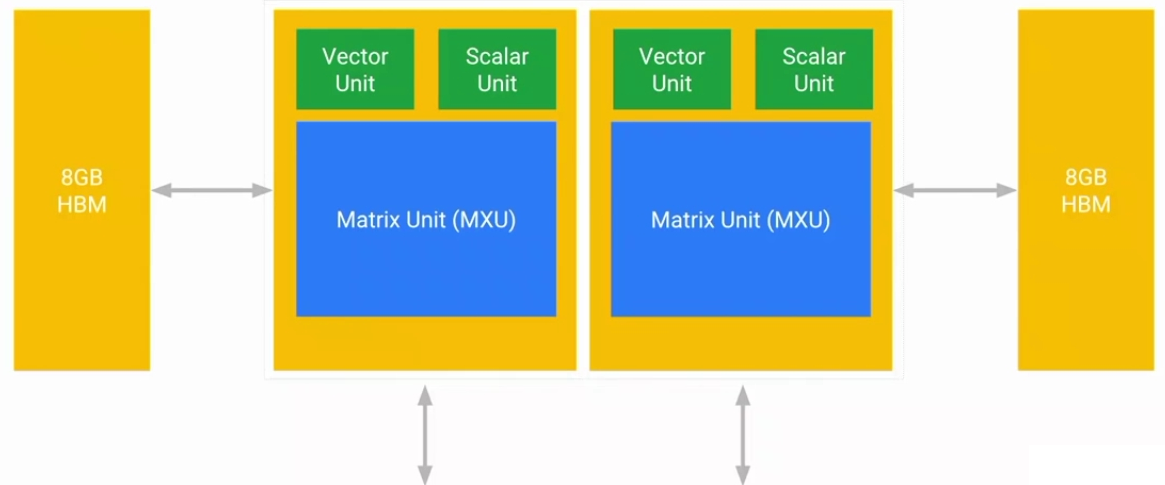
\includegraphics[scale=.255]{images/10chiplayout.png}
            \caption
            {10. Cloud TPU chip layout}
            \label{fig: cloud TPU chip layout}
        
  \end{minipage}}
\end{figure}
  \end{frame}
  %%%%%%%%%%%%%%%%%%%%%%%%%%%%%%%%%%%%%%%%%%%%%%%%%%%%%%
  
  \begin{frame} [c]
  \frametitle{Architechture : Cloud TPU}
			\begin{figure}[ht]
  {\begin{minipage}[t]{120pt}
    \includegraphics[height=100pt,width=150pt]{test}
    	\begin{itemize}
		\justifying
		{\small \item22.5 TFLOPS per core
\item 2 core per chip
\item 4 chips per 150 TFLOP cloud TPU
\item Scalar unit
\item Vector unit
\item Matrix unit
\item Mostly float 32

	}

		\end{itemize}		
  \end{minipage}}
  \hfill
  {\begin{minipage}[t]{190pt}
    \includegraphics[height=60pt,width=150pt]{test}
    
                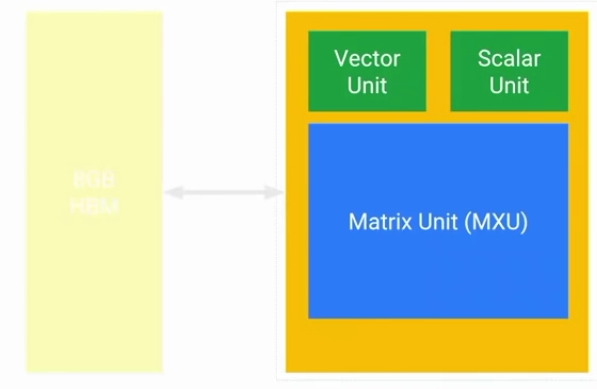
\includegraphics[scale=.37]{images/11chiplayoutcore.png}
            \caption
            {11. Cloud TPU chip layout core}
            \label{fig: cloud TPU chip layout core}
        
  \end{minipage}}
\end{figure}
  \end{frame}
  %%%%%%%%%%%%%%%%%%%%%%%%%%%%%%%%%%%%%%%%%%%%%%%%%%%%%%
  \begin{frame} [c]
  \frametitle{Architechture : Cloud TPU}
			\begin{figure}[ht]
 {\begin{minipage}{170pt}
    \includegraphics[height=100pt,width=150pt]{test}
    	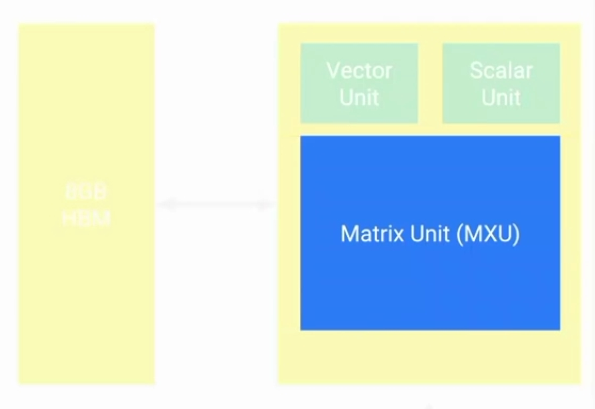
\includegraphics[scale=.34]{images/12chiplayoutcore.png}
            \caption
            {12. Cloud TPU chip layout}
            \label{fig: cloud TPU chip layout core}		
  \end{minipage}}
  %hfill
  {\begin{minipage}[b]{130pt}
    \includegraphics[height=500pt,width=150pt]{test}
    
    \begin{itemize}
		\justifying
		{\small \item Matrix Unit (MXU)
128 x 128 systolic array
  \item bfloat16 multiplies
\item Float32 accumulate	}
		\end{itemize}
  \end{minipage}}
  \linebreak
  \linebreak
  \linebreak
  	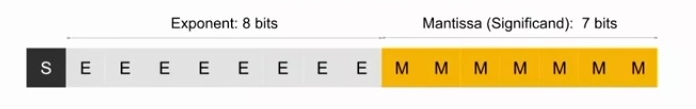
\includegraphics[scale=.5]{images/13chiplayout.png}
            \caption
            {13. bfloat16 - Brain Floating Point Format}
            \label{fig: bfloat16}
\end{figure}
  \end{frame}
 
	%%%%%%%%%%%%%%%%%%%%%%%%%%%%%%%%%%%%
	\section{COMPARISON}               
    \begin{frame} [c]
    \frametitle{CPU Vs GPU Vs TPU}
\begin{figure}[ht]
  {\begin{minipage}[t]{105pt}
    \includegraphics[height=100pt,width=150pt]{test}
    \begin{center}{\LARGE \textbf{CPU}}\newline
    {\footnotesize (Central processing unit)}
    \end{center}
    \begin{itemize}
        \item  Low Latency 
        \item Low Throughput
        \item Scalar Operations
\end{itemize}
  \end{minipage}}
  \hfill
  {\begin{minipage}[t]{112.5pt}
    \includegraphics[height=60pt,width=150pt]{test}
    \begin{center}{\LARGE \textbf{GPU}}\newline
    {\footnotesize (Graphical processing unit)}
    \end{center}
    \begin{itemize}
        \item  high latency
        \item high throughput [matrix multiplication]
        \item Vector Operations
    \end{itemize}
  \end{minipage}}
  {\begin{minipage}[t]{118pt}
    \includegraphics[height=100pt,width=150pt]{test}
    \begin{center}{\LARGE \textbf{TPU}}\newline
    {\footnotesize (TensorFlow processing unit)}
    \end{center}
    \begin{itemize}
        \item Tpu  use systolic matrix multiplication
        \item very high throughput 
        \item bfloat16
        \item TPU delivers 15–30X more throughput than contemporary CPUs and GPUs,
        \end{itemize}
  \end{minipage}}
\end{figure}
	\end{frame}
	%%%%%%%%%%%%%%%%%%%%%%%%%%%%%%%%%%%%%
	\begin{frame}{Operations per Cycle}
	\begin{center}
	{\large \textbf{Number of operations per cycle between CPU, GPU and TPU}}
	\linebreak
	\end{center}
	\begin{table}
	\begin{tabular}{p{5.5cm} p{5.5cm}}
	\hline
	CPU \linebreak & a few   \\
	\hline
	CPU (vector extension) & tens \linebreak \\
	\hline
	GPU \linebreak & tens of thousands  \\
	\hline
	TPU \linebreak & hundereds of thousands, upto 128k\\
	\hline
	\end{tabular}
	\caption{2.Operations per cycle}
	 \label{tab:tab2}
	\end{table}
	\end{frame}
	
	%%%%%%%%%%%%%%%%%%%%%%%%%%%%%%%%%%%%
	\begin{frame}{Comparing CPU, GPU and TPU}
	\begin{figure}
            \centering
            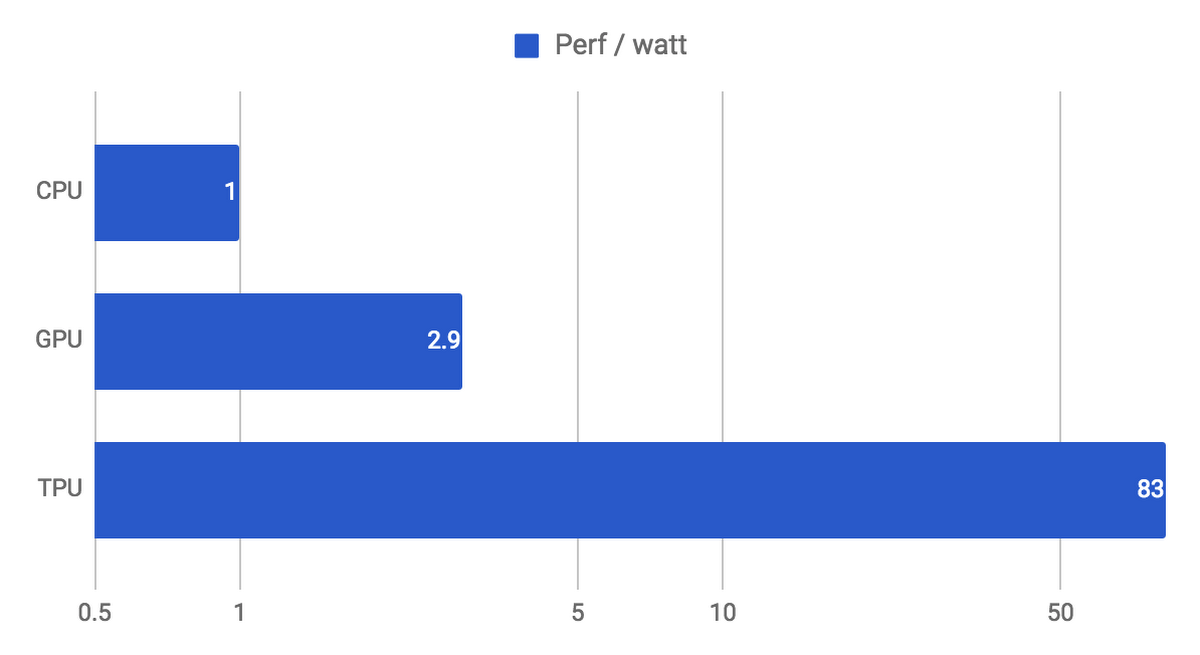
\includegraphics[scale=.36]{images/14pre.png}
            \caption{14. Performance / watt, relative to contemporary CPUs and GPUs (Incremental, weighted mean) (in log scale) }
            \label{graph:performance per watt}
        \end{figure}
	    
	\end{frame}
	%%%%%%%%%%%%%%%%%%%%%%%%%%%%%%%%%%%%
	\begin{frame}{Comparing CPU, GPU and TPU}
	\begin{figure}
            \centering
            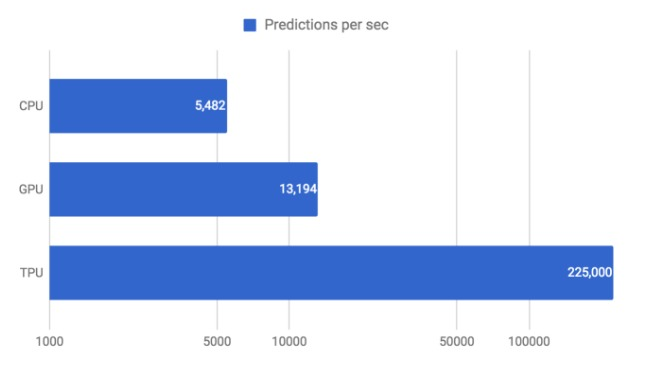
\includegraphics[scale=.65]{images/15pre.png}
            \caption{15.Throughput under 7 ms latency limit (in log scale) }
            \label{graph:prediction per sec}
        \end{figure}
	    
	\end{frame}
	%%%%%%%%%%%%%%%%%%%%%%%%%%%%%%%%%%%%
	
\section{PERFORMANCE ANALYSIS}
    \begin{frame}
    \frametitle{Performance Analysis}
        \begin{figure}[h]
 \hfill
\begin{subfigure}[b]{0.486\textwidth}
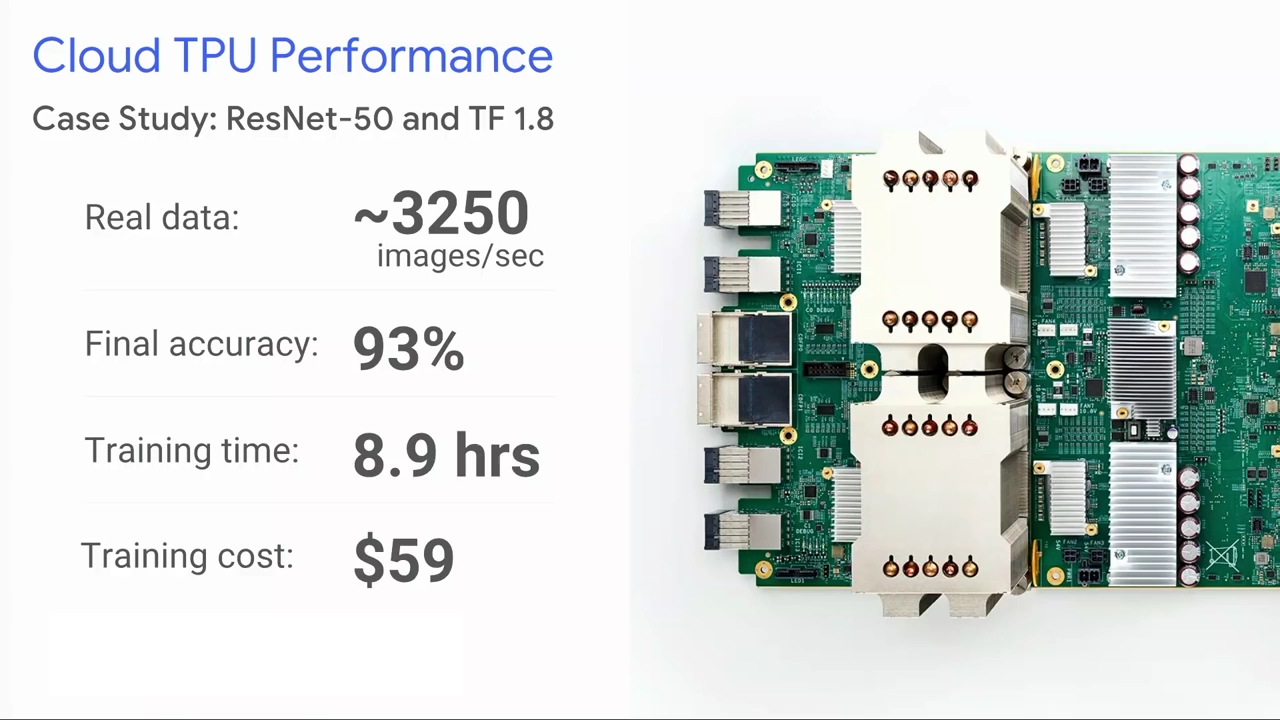
\includegraphics[width=\linewidth]{images/16aperformance.png}
\caption{ Cloud TPU}
\label{fig:TPUv3 pod}
\end{subfigure}
\hspace{0.1cm}
\begin{subfigure}[b]{0.486\textwidth}
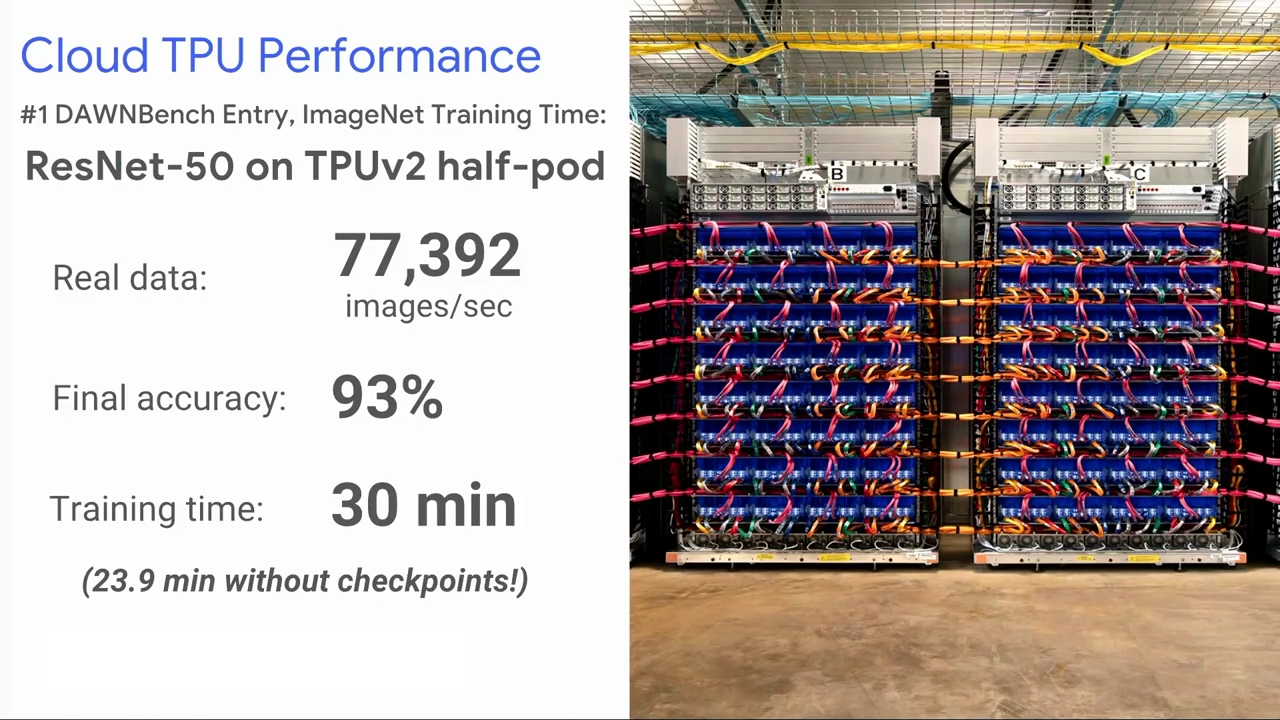
\includegraphics[width=\linewidth]{images/16bperformance.png}
\caption{Cloud TPU pod}
\label{fig:TPUv3 Chip}
\end{subfigure}
\caption{16. Performance Analysis}
\label{fig:TPUv3}
\end{figure}
    \end{frame}
%%%%%%%%%%%%%%%%%%%%%%%%%%%%%%%%%%%%%%%%%%%%%%%%%%%%%%%%
\section{PERFORMANCE ANALYSIS}
    \begin{frame}
    \frametitle{Scaling}
        \begin{figure}[h]
 \hfill
\begin{subfigure}[b]{0.49\textwidth}
\includegraphics[width=\linewidth]{images/17bscaling.png}
\caption{Performance}
\label{fig:TPUv3 pod}
\end{subfigure}
\begin{subfigure}[b]{0.49\textwidth}
\includegraphics[width=\linewidth]{images/17ascaling.png}
\caption{Accuracy}
\label{fig:TPUv3 Chip}
\end{subfigure}
\caption{17. Scaling }
\label{fig:TPUv3}
\end{figure}
    \end{frame}
%%%%%%%%%%%%%%%%%%%%%%%%%%%%%%%%%%%%%%%%%%%%%%%%%%%%%%%%

   \section{ADVANTAGES OF CLOUD}
    	\begin{frame}
		\frametitle{Google Cloud advantages over on-prem hosting}
		\begin{figure}[ht]
  {\begin{minipage}[t]{90pt}
  \begin{center}
    \includegraphics[height=100pt,width=150pt]{test}
    \includegraphics[scale=.4]{images/18a.png}\newline
    \newline {\scriptsize
    \textbf{Top-notch infrastructure }\newline
    Mix and match the components you need}
    \end{center}
  \end{minipage}}
  \hfill
  {\begin{minipage}[t]{71.5pt}
  \begin{center}
    \includegraphics[height=60pt,width=150pt]{test}
    \includegraphics[scale=.4]{images/18b.png}\newline
    \newline {\scriptsize
    \textbf{Faster provisoning }\newline
    Scale up quickly as your needs change}
    \end{center}
  \end{minipage}}
  {\begin{minipage}[t]{71.5pt}
  \begin{center}
    \includegraphics[height=100pt,width=150pt]{test}
     \includegraphics[scale=.4]{images/18c.png}\newline
    \newline {\scriptsize
    \textbf{Security built-in }\newline
    Powerful tools for data access \& user control}
     \end{center}
  \end{minipage}}
  \hfill
  {\begin{minipage}[t]{98.8pt}
  \begin{center}
    \includegraphics[height=60pt,width=150pt]{test}
     \includegraphics[scale=.4]{images/18d.png}\newline
    \newline {\scriptsize
    \textbf{Reduce capital expenditure }\newline
    On-demand pricing, pray only for what you need}
     \end{center}
  \end{minipage}}
\end{figure}
	\end{frame}
%%%%%%%%%%%%%%%%%%%%%%%%%%%%%%%%%%%%%%%%%%%%%%%%%%%%%%%%%%	
	\section{USING CLOUD TPU}
	\begin{frame}
	\frametitle{Using Cloud TPU}
	\begin{center}\textbf{ Cloud TPUs are network attached}
	\begin{figure}
            \centering
            \includegraphics[scale=.36]{images/19usingcloudtpu.png}
            \caption{19. Using Cloud TPUs }
            \label{graph:performance per watt}
        \end{figure}
        \linebreak
{\small \textbf{No drivers to install} - just use \linebreak the machine images they provide!}
\end{center}
	\end{frame}
	%%%%%%%%%%%%%%%%%%%%%%%%%%%%%%%%%%%%%%%%%%%%%%%%
	\begin{frame}{Cloud TPU pricing}
	\begin{table}
	\hfill
	\begin{tabular}{|p{3.6cm}|| p{3.5cm}||p{3.5cm}|}
	\hline

	{\small \textbf{\newline Google Cloud Region \newline}}  & {\small \textbf{\newline Normal(hourly)}} & {\small \textbf{\newline Preemtible(hourly)}} \\
	\hline \hline
	{\small US-central1 \newline} & {\small 4.50\$/hour}& {\small 1.35\$/hour} \\
	\hline
	{\small europe-west4 \newline} & {\small 4.95\$/hour} &  {\small 1.485\$/hour}  \\
	\hline
{\small east-asia1 \newline} & {\small 5.22\$/hour} & {\small 1.566\$/hour} \\
	\hline
	\end{tabular}
	\caption{3. Cloud TPU pricing}
	 \label{tab:tab3}
	\end{table}
	\end{frame}
	%%%%%%%%%%%%%%%%%%%%%%%%%%%%%%%%%%%%%%%%%%%%%%%%%%%%
	\begin{frame}{Available reference models for Cloud TPUs}
	\begin{figure}[ht]
  {\begin{minipage}[t]{89pt}
    \includegraphics[height=100pt,width=150pt]{test}
    \includegraphics[scale=.37]{images/20a.png}\newline
    \newline {\scriptsize
    \textbf{Image Recognition: }\newline
    AmoebaNet-d \newline
ResNet-50/101/152/200 \newline
Inception v2/v3/v4 \newline
DenseNet
\linebreak 

    \textbf{Object Detection: }\newline
     RatinaNet \newline
     \linebreak
\textbf{low-Resourse model:}\newline
MobileNet \newline
SqueezeNet \newline
}
  \end{minipage}}
  \hfill
  {\begin{minipage}[t]{97pt}
    \includegraphics[height=60pt,width=150pt]{test}
    \includegraphics[scale=.35]{images/20b.png}\newline
    \newline {\scriptsize
    \textbf{Models: }\newline
    Machine translation\newline
Language modeling\newline
Sentimental analyzing\newline
Question-answering\newline
(all Transformer-based)

   }
  \end{minipage}}
  {\begin{minipage}[t]{58pt}
    \includegraphics[height=100pt,width=150pt]{test}
    \includegraphics[scale=.37]{images/20c.png}\newline
    \newline {\scriptsize
    \textbf{Models: }\newline
    ASR Transform\newline
(LibriSpeech)
}
  \end{minipage}}
  \hfill
  {\begin{minipage}[t]{60pt}
    \includegraphics[height=60pt,width=150pt]{test}
    \includegraphics[scale=.37]{images/20d.png}\newline
    \newline {\scriptsize
    \textbf{Models:}\newline
    Image Transform\newline
DCGAN}
  \end{minipage}}
\end{figure}
	    
	\end{frame}
	%%%%%%%%%%%%%%%%%%%%%%%%%%%%%%%%%%%%%%%%%%%%%%%%%%%%%%%
	\begin{frame}{Advantages of reference models}
	\begin{itemize}
	    \item High performance
\item Open source
\item Cutting-edge model architectures
\item Continuously tested for performance
\item Continuously tested for accuracy
\item Get up  and running quickly, modified as needed
\item Train and run on your data
	\end{itemize}
	\end{frame}
	%%%%%%%%%%%%%%%%%%%%%%%%%%%%%%%%%%%%%%%%%%%%%%%%%%%%%%%%%%
	

	
	\section{REFERENCES}
	\section*{Bibliography}
	
	%%%%%%%%%% Bibliography %%%%%%%%%%%%
	
	\begin{frame}[<1->][allowframebreaks]
		\frametitle{References}		
		\nocite{*}
		% experiment with different styles if you want to. I am just using plain style.
		\bibliographystyle{plain}
		% see a file called 103.bib in the folder. That is where you put your references.
		{\small \bibliography{103}}
	\end{frame}
	
%	\begin{frame}[c]
%	\includegraphics[scale=.7]{thnk.PNG}
%	\end{frame}
	
\end{document}
